\chapter{Literature Review}

\textit{``Hunger roared up in him like a hopeless lust.\\ 
He walked the ship as though following a chart. Up. Down. Across. Back. Stem. Port. Stern. Starboard. The churning of the waves. \\
The ropes clanking on the masts. The blind of salt water. The wind ripping at the sails.''\\
\textemdash\ ``Star of the Sea'' by Joseph O'Connor}
\vspace{.2cm}

\section{A Brief Famine Outline}

The Irish lumper potato with its excellent ability to grow in poor and wet soils, was the predominant potato variety in pre-famine Ireland. It was introduced to U.K. around 1806 \citep{tucker2016potato}, and rapidly replacing almost all other varieties in the recipes of the poor. Usually, on account of its intolerance of frost, the farmer sows in March or April, and the first early potatoes will be harvested in June, followed by the second early potatoes in July, and the third not later than October. With a 1.32 \% growth in lower class per year in Ireland from the centennial before 1841, in 1845 about 32\% of the arable land in Ireland was already under potato cultivation \citep{solar2015ireland}.

The first record of late blight on potatoes in Ireland is thought to be Dr Lindley's letter in September 16, 1845, with his concern words, he wrote: ``The potato murrain has unequivocally declared itself in Ireland, where will Ireland be in the event of a universal potato rot''? \citep{kelly1995great}. Things were getting worse in next year, a government documents collection book recorded that: ``the poor Irish lost their potatoes again'' (1 September, 1846) so that ``Many, full many, must this winter leave their homes, and traverse the country in quest of work'' (15 September, 1846). Government employee pointed out a fact, ``to maintain Ireland's population, her agriculture must be greatly improved'' (31 October, 1846). But soon the famine was spiraling out of control, in newspaper's leading article, reporter wrote: ``eye-witnesses of scores and hundreds of poor creatures actually dying for want a meal'' (8 March, 1847).  which caused a ``immigration in poor Irish people'' (November 10, 1847) and ``disorder in Ireland'' (November 13, 1847) and finally, Ireland faced a situation that ``Labour is the first price and is the source of all wealth'' (December 30, 1847) \citep{times1880famineletter}.

In January 1847, the government pushed for reform of the Poor Law, which exacerbated the ravages of famine in Ireland \textendash\ particularly in the south and west of Ireland. The Poor Law was introduced in Ireland in July 1838 and provided for the establishment of 130 trade unions throughout Ireland, the poor of which were to be relieved and regulated by the guardians of the trade unions \citep{o1985new}. It is very difficult to objectively assess the role of poverty law, which on the one hand does provide relief to many poor people, but on the other hand is also characterized by Foucault's theory of power genealogy like ``micro-power'' and the operation of ``bio-politics''.

\begin{itemize}
    \item [] \textit{It is true we have been careful not to put forward a poor-law as a mean to supply, but have claimed for it only a place among the means of distributing supplies \textendash\ of promoting employment, and of enforcing upon poverty the care and protection of the labour. Still, if that surplus of unfilled mouths is to be always in front of us, it must be confessed that very little good, after all, will be accomplished.} \citep{thomas1847poorlaw}
\end{itemize}


From the census data of 1841 and 1851 (Figure 2.1), we can calculate the change in population of the different provinces after the famine, which showed the result that the west and south suffered far more from famine than the east and north. The five counties with the greatest decreases in population are Donegal, Connaught, in the west, 279,601; Cork, Munster, in the south, 209,822; Galway, Connaught, in the west, 125,026; Tipperary, Munster, in the south, 103,986, and Roscommon, Connaught, in the west, 80,155.\ \textit{The freeman's journal} similarly supports this conclusion in its April 27, 1847 article documenting the damage to parishes including Killedy, Toomavara, Abbey, Lorha and Dorrow, etc \citep{freeman1847parishes}.

\begin{figure}[h]
    \centering
    \caption{County Population 1841 \textendash\ 1851}
    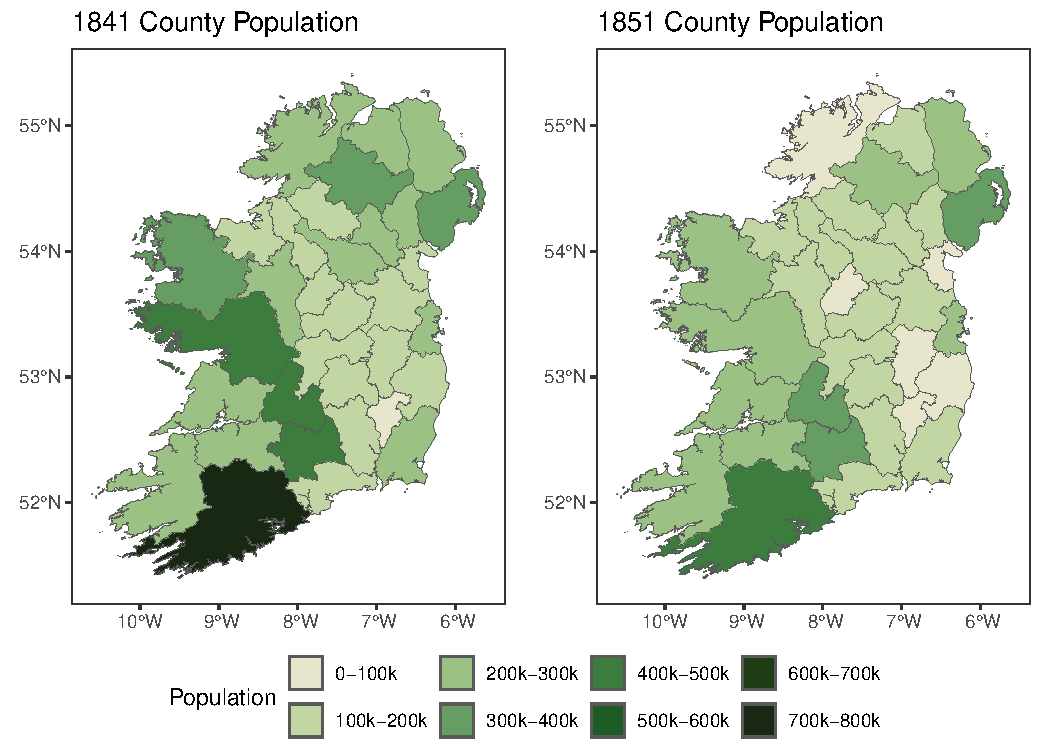
\includegraphics[width=.95\textwidth]{../03_outputs/map1841_1851.pdf}
\end{figure}


\section{Refuting some hypotheses}

This part I will refute some hypothesis of famine origin. Many people regard single factor as the root of the Great Famine.

\begin{figure}[h]
    \centering
    \caption{Food Structure}
    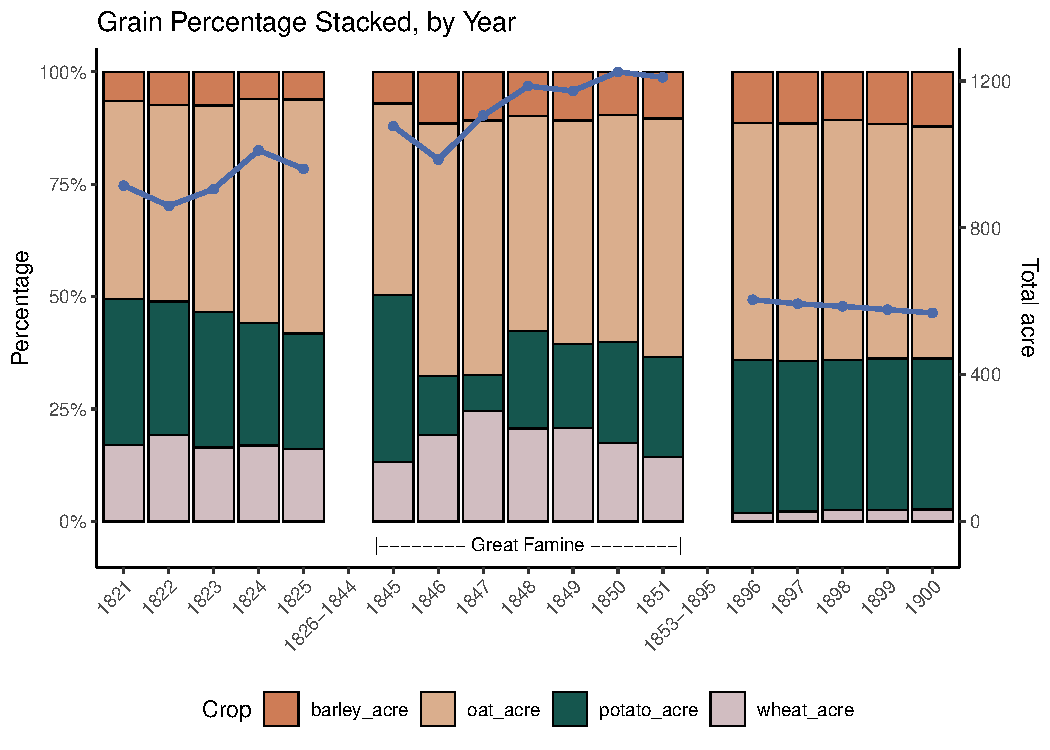
\includegraphics[width=.95\textwidth]{../03_outputs/food_structure.pdf}
\end{figure}

\subsection{Potato Blight}

In Nature journal,

1845 June Belgium, August France, August South of UK, September Ireland

\begin{figure}[h]
    \centering
    \caption{Food Structure}
    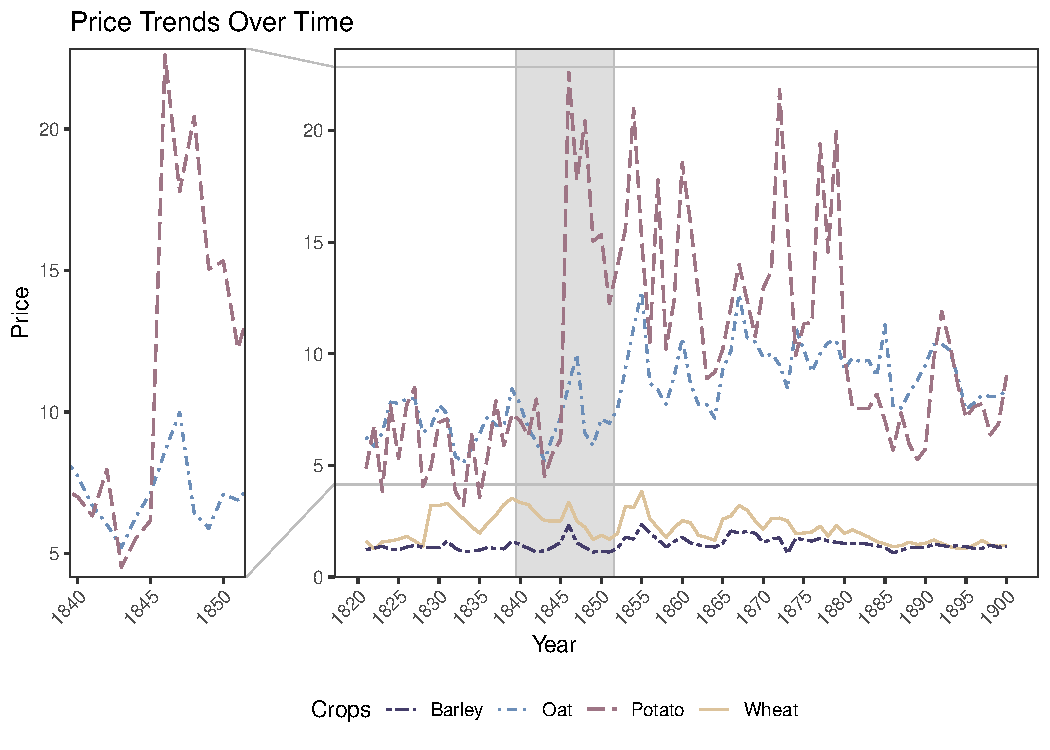
\includegraphics[width=.95\textwidth]{../03_outputs/grain_price.pdf}
\end{figure}



1. Blame potato blight as the only origin of famine

People believe potato blight was responsible for the Irish Great Famine. 

lumper potato

Blight became a semi-permanent fixture until the end of the century, when effective treatments were found \citep{o1994economic}.

2. Ireland have the bad land quality.

\section{Entitlement Approach}



I n the field of famine studies, scholars as diverse asSusan George (1980), Amartya Sen (1981, 2000),Michael Watts (1983), Amrita Rangasami (1985),and Stephen Devereux (2001) have argued that faminesdo not necessarily begin with crop failures, droughts, orequivalent climatic hazards. On the contrary, their vi-olence is coordinated much earlier when a populationis progressively brought to the point of collapse. Readthis way, a crop failure, or indeed a drought, is simply an“environmental trigger” in a much larger narrative of ag-gregated poverty and mass vulnerability (George 1984;Devereux 2002). Despite the fact that the Great IrishFamine is now a major field of scholarly enquiry, therehas been very little attempt to engage with these criti-cal perspectives—derived primarily from famine expe-riences in the global South—nor has there been any at-tempt to analyze the Great Famine from the perspectiveof colonial governance and population management. \citep{nally2008coming}


I will operationalize entitlement approach into these 4 dimensions according to the book:

(1) trade-based entitlement: price, grain amount, 

(2) production-based entitlement: tax policy

(3) own-labour entitlement: wage, land own amount, poor law

(4) inheritance and transfer entitlement: none, hard to get data






